%
\section{Option 2: converter inside the OPA}
\label{section:geometry_v4}
If the converter radius is large enough, the converter ring surrounding the pion degrader
could start limiting the degrader arm movement. 
Therefore, becomes attractive to consider positioning the converter inside the OPA,
and have is supported by the OPA. In this case, a gold converter foil could be put
on a thin carbon foam ring supported by the OPA, similar to the stopping target.
That might allow to increase the width of the converter ring, increasing the yield
of $\gamma \to e^+e^-$ events respectively. That would also simplify the geometry
of the moving part of the degrader inside the narrow gap in between the TS and the OPA.

\begin{figure}[H]
  \begin{tikzpicture}
    \node[anchor=south west,inner sep=0] at (0,0.) {
      % \node[shift={(0 cm,0.cm)},inner sep=0,rotate={90}] at (0,0) {}
      \makebox[\textwidth][c] {
        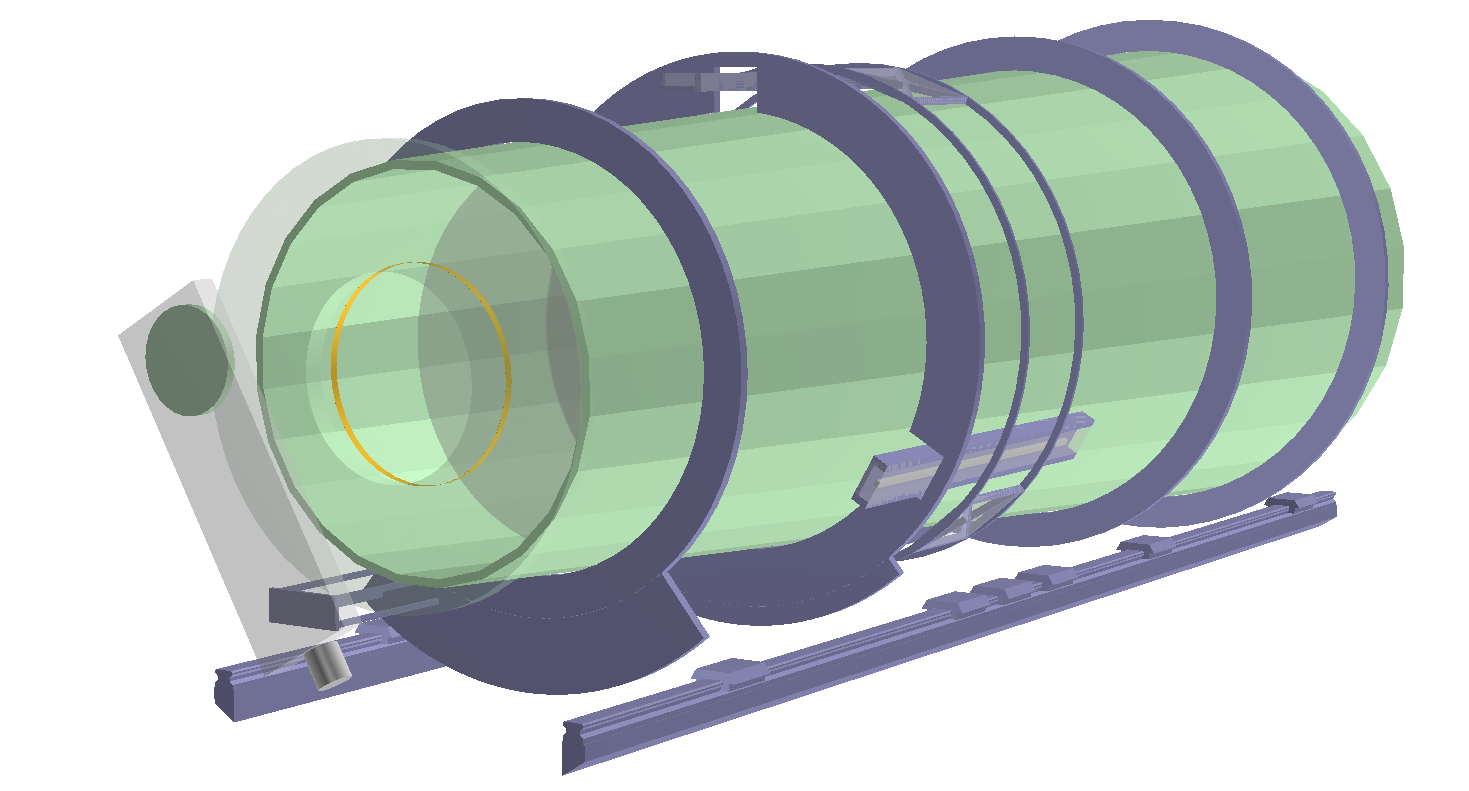
\includegraphics[width=0.90\textwidth]{png/pipenu_cele3b0_geom_degrader}
      }
    };
    % \node [text width=8cm, scale=1.0] at (14.5,0.5) {$\mu_B$, expected background mean};
    % \node [text width=8cm, scale=1.0, rotate={90}] at (1.5,7.5) { $S_{D}$, ``discovery'' signal strength  };
  \end{tikzpicture}
  \caption{
    \label{figure:degrader_v4}
    degrader v4: converter ring supported by OPA. The carbon foam ring is not shown.
  }
\end{figure}

%%%%%%%%%%%%%%%%%%%%%%%%%%%%%%%%%%%%%%%%%%%%%%%%%%%%%%%%%%%%%%%%%%%%%%%%%%%%%%
\newpage
\subsection{Parameters used in the simulation}

\begin{itemize}
\item
  pion stops: reuse pipenu:bpim01b0s24r000, {\red for the next iteration re-simulate the beam properly}
\item
  converter foil:  thickness = 100$\mu$, width = 2 cm, $R_{out} = 250$ mm
\item
  carbon foam is not included into the simulation. The approximation is justified
  by the fact that 1cm thick layer of carbon foam, in units of radiation length,
  adds much less material than a 100 um thick gold foil.
\item 
  simulation of RPC photons:
  \begin{itemize}
  \item 
    degrader material: CH2 , 24mm thick,
    to approximately match the material of 4mm-thick Ti converter.
  \item 
    \red{need to re-optimize the thickness to match the pion stopping rate
    at the ST to that of 4mm Ti}
  \end{itemize}
\item
  generated statistics: 10M single $\gamma$ events, $E_\gamma = 129.4$ MeV, 
\item
  simulated range of cos(theta): [0,0.45] 
\item
  dataset family: pipenu:rpc07b0
\end{itemize}

%%%%%%%%%%%%%%%%%%%%%%%%%%%%%%%%%%%%%%%%%%%%%%%%%%%%%%%%%%%%%%%%%%%%%%%%%%%%%%
\newpage
\subsection{Resolution in the reconstructed photon energy}

The distribution of $E_\gamma = P(e^+) + P(e^-)$ for the events
with the reconstructed $e^+$ and $e^-$ tracks is shown in Figure~\ref{figure:t2_0_smom_1}.
Overlaid is the fit of the distribution with the SU2020 resolution function
defined by Eq.~\ref{eq:dio_mom_res}.
The $\chi^2/DOF$ of the fit is close to one, and with about 1000 events in the peak,
the uncertainty on the peak position returned by the fitter is below 10 keV/c.
This is a good indication that statistics of 1000 events should be sufficient
for calibrating the momentum scale with the accuracy better than 100 keV/c.

Although the track topology in $\gamma \to e^+e^-$ events is different from
$\sim$ 100 MeV/c CE tracks, together with the reconstructed \piplusenu\ peak,
this calibration should yield a conclusive determination of the Mu2e momentum scale.

\begin{figure}[H]
  \begin{tikzpicture}
    \node[anchor=south west,inner sep=0] at (0,0.) {
      % \node[shift={(0 cm,0.cm)},inner sep=0,rotate={90}] at (0,0) {}
      \makebox[\textwidth][c] {
        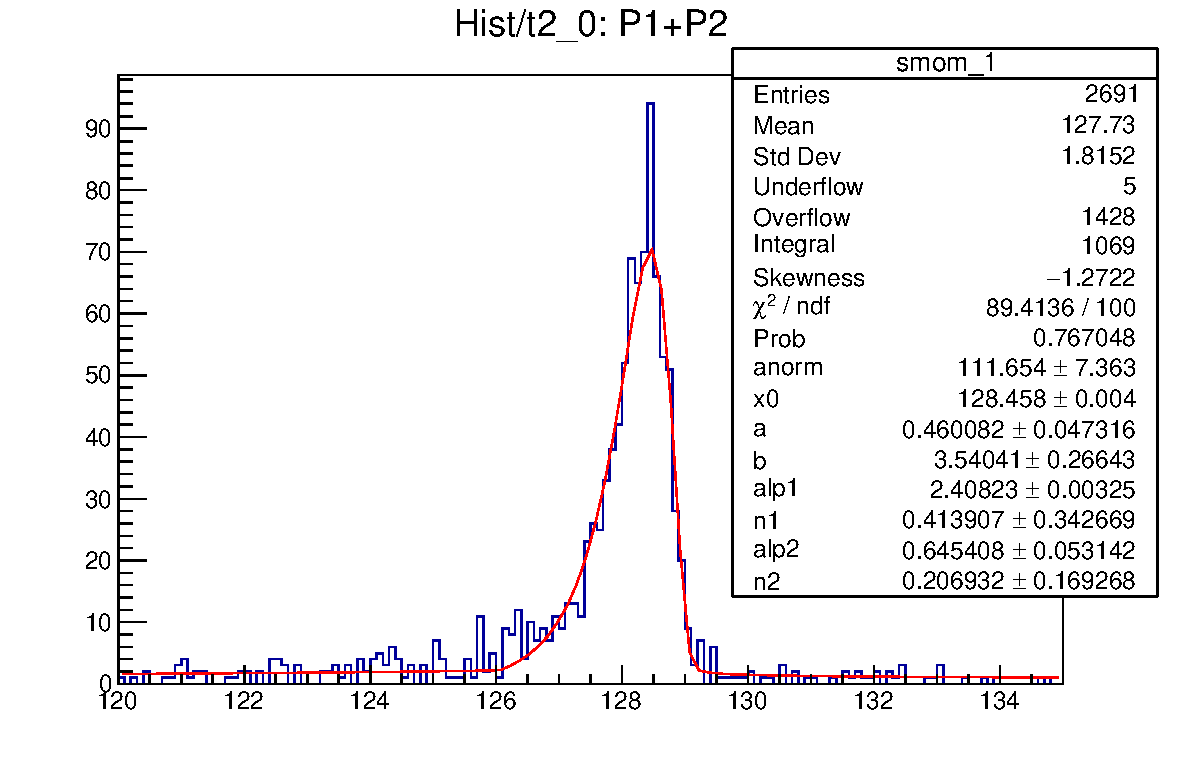
\includegraphics[width=0.95\textwidth]{pdf/figure_00082}
      }
    };
    % \node [text width=8cm, scale=1.0] at (14.5,0.5) {$\mu_B$, expected background mean};
    % \node [text width=8cm, scale=1.0, rotate={90}] at (1.5,7.5) { $S_{D}$, ``discovery'' signal strength  };
  \end{tikzpicture}
  \caption{
    \label{figure:t2_0_smom_1}
    Distribution of $E_\gamma = P(e^+) + P(e^-)$ for events with two reconstructed tracks
  }
\end{figure}

%%%%%%%%%%%%%%%%%%%%%%%%%%%%%%%%%%%%%%%%%%%%%%%%%%%%%%%%%%%%%%%%%%%%%%%%%%%%%%
\newpage
\subsection{Converter impact on the CE acceptance}

To estimate impact of the converter foil positioned permanently in the DS  
volume on the CE acceptance, two single particle datasets,
with and without the converter, have been generated

\begin{itemize}
\item
  dataset families: pipenu:cele0b0 (default geometry) and pipenu:cele3b0 (converter added)
\item 
  CE simulation: Al. LL rad corrections
\item
  2.5M events per configuration.
\item 
  perfect detector model - no mis-calibrations, no misalignment
\end{itemize}

Figure~\ref{figure:ce_momentum_tsda} compares the acceptances
for the two simulated configurations.
%
Plotted are the momentum distributions for all reconstructed CE tracks,
no selections applied.

For the momentum window of [103,105] MeV/c, an introduction of a
100 um thick and 2cm wide Au converter at R = 250 mm reduces
the CE acceptance by 0.16\%.

\begin{figure}[H]
  \begin{tikzpicture}
    \node[anchor=south west,inner sep=0] at (0,0.) {
      % \node[shift={(0 cm,0.cm)},inner sep=0,rotate={90}] at (0,0) {}
      % \makebox[\textwidth][c] {
        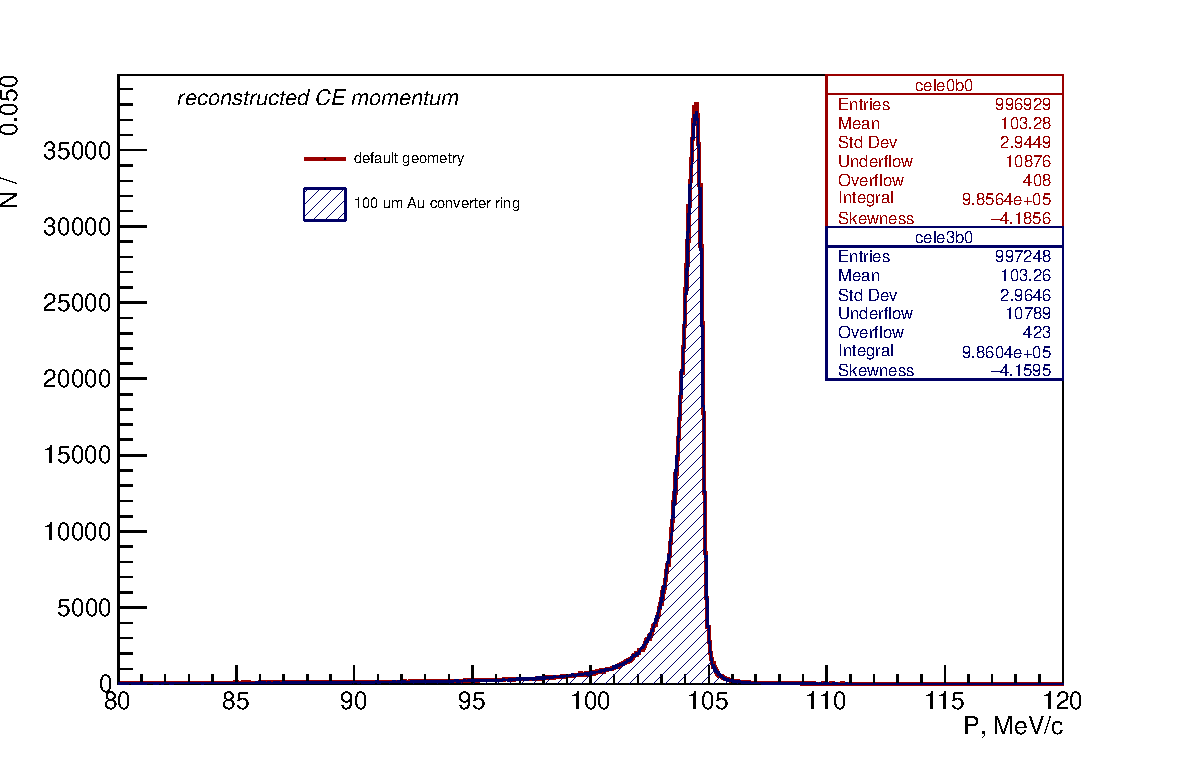
\includegraphics[width=0.54\textwidth]{pdf/figure_00051}
      % }
    };
    \node[anchor=south west,inner sep=0] at (9.8,0.) {
      % \node[shift={(0 cm,0.cm)},inner sep=0,rotate={90}] at (0,0) {}
      % \makebox[\textwidth][c] {
        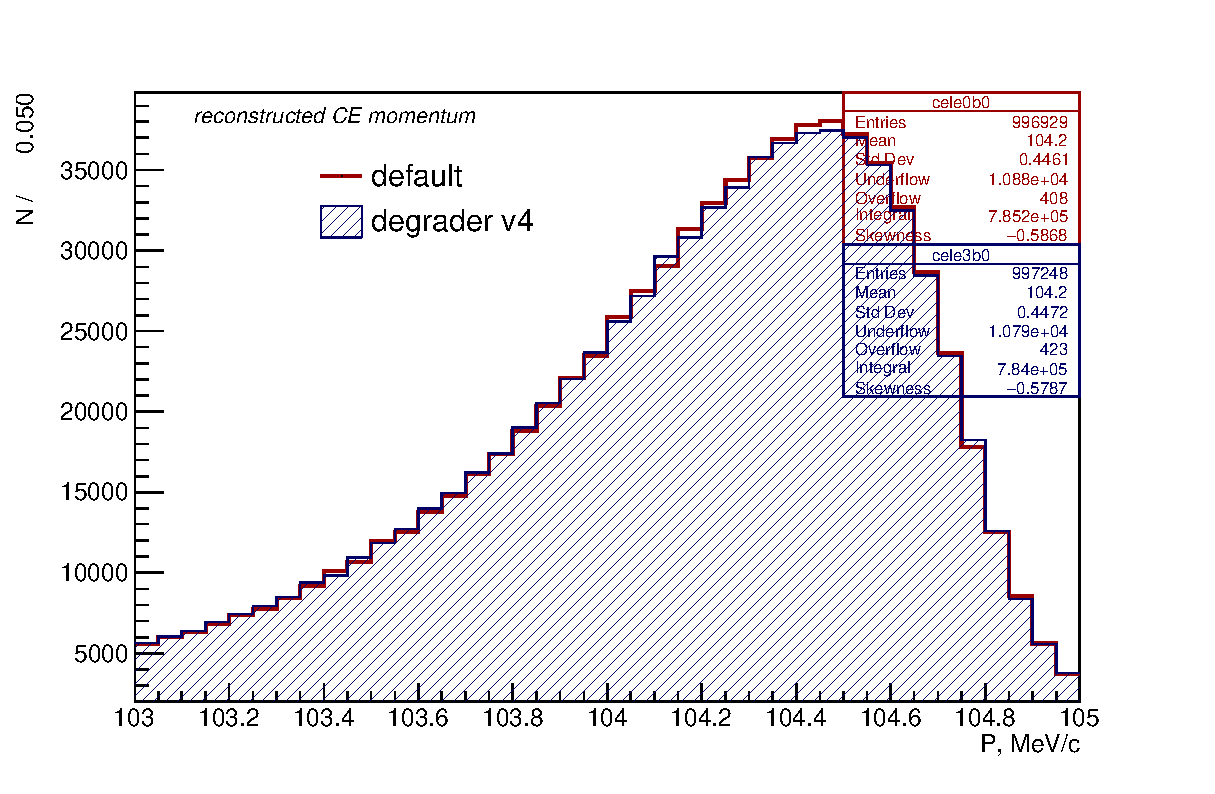
\includegraphics[width=0.54\textwidth]{pdf/figure_00052}
      % }
    };
    % \node [text width=8cm, scale=1.0] at (14.5,0.5) {$\mu_B$, expected background mean};
    % \node [text width=8cm, scale=1.0, rotate={90}] at (1.5,7.5) { $S_{D}$, ``discovery'' signal strength  };
  \end{tikzpicture}
  \caption{
    CE momentum distribution for two geometries, with and without the converter ring. 
  }
  \label{figure:ce_momentum_tsda}
\end{figure}
%%% Local Variables:
%%% mode: latex
%%% TeX-master: t
%%% End:
